%% This work may be distributed and/or modified under the conditions of the LaTeX Project Public License, either version 1.3 of this license or (at your option) any later version. The latest version of this license is in http://www.latex-project.org/lppl.txt and version 1.3 or later is part of all distributions of LaTeX version 2005/12/01 or later. This work has the LPPL maintenance status `maintained'. Further information about abnTeX2 are available on https://github.com/abntex/abntex2 | https://www.abntex.net.br/
%%
%% The Current maintainer of this template is Geraldo Pereira de M. Jr. 
%% Contact: geraldo.pmj@gmail.com
%%
\documentclass[
	12pt,				% tamanho da fonte
	oneside,			% impressão em um lado da folha (relatório entregue em PDF)
	a4paper,			% tamanho do papel.
	sumario = tradicional,
	english,			% idioma adicional para hifenização
	brazilian			% o último idioma é o principal do documento
	]{abntex2}
% ---
% Pacotes básicos 
% --
\usepackage{times} %{lmodern}	% Usa a fonte Latin Modern			
\usepackage[T1]{fontenc}% Selecao de codigos de fonte.
\usepackage[utf8]{inputenc}% Codificacao do documento (conversão automática dos acentos)
\usepackage{indentfirst}	% Indenta o primeiro parágrafo de cada seção.
\usepackage[top=30mm, bottom=20mm, left=30mm, right=20mm]{geometry}
\usepackage{color}		% Controle das cores
\usepackage{graphicx}	% Inclusão de gráficos
\graphicspath{ {./build/figuras/} }
\usepackage{microtype} 	% para melhorias de justificação
\usepackage{fancyhdr} %define o estilo do documento
\usepackage{array} %permite o uso de tabelas
\usepackage{longtable} %permite o uso de tabelas personalizadas
\usepackage{rotating} %permite rotacionar imagens
\usepackage{tikz} %permite o desenho de formas geométricas simples dadas suas características
\usepackage{PPGAN}
\usepackage{ragged2e}
\usepackage{csquotes}
\usepackage{pdfpages}
\usepackage{amsmath}
\usepackage{amssymb}
% ---
% Pacotes de citações
% ---
\usepackage[style=abnt, repeatfields, backend=biber]{biblatex}
\addbibresource{referencias.bib} % Seus arquivos de

\ifthenelse{\equal{\ABNTEXisarticle}{true}}{%
\renewcommand{\maketitlehookb}{}
}{}
\PassOptionsToPackage{brazilian,english}{babel}

\DeclareUnicodeCharacter{031C}{ç}


% ---
% Configurações de aparência do PDF final

% alterando o aspecto da cor azul
\definecolor{blue}{RGB}{41,5,195}

% informações do PDF
\makeatletter
\hypersetup{
     	%pagebackref=true,
		pdftitle={\@title}, 
		pdfauthor={\@author},
    	pdfsubject={\imprimirpreambulo},
	    pdfcreator={\@author},
		pdfkeywords={palavra-chave}{palavra-chave}{palavra-chave}, 
		colorlinks=true,       		% false: boxed links; true: colored links
    	linkcolor=black,          	% color of internal links
    	citecolor=black,        		% color of links to bibliography
    	filecolor=magenta,      		% color of file links
		urlcolor=black,
		bookmarksdepth=4}
\makeatother
% --- 

% ---
% Posiciona figuras e tabelas no topo da página quando adicionadas sozinhas
% em um página em branco. Ver https://github.com/abntex/abntex2/issues/170
\makeatletter
\setlength{\@fptop}{5pt} % Set distance from top of page to first float
\makeatother
% ---

% ---
% Possibilita criação de Quadros e Lista de quadros.
% Ver https://github.com/abntex/abntex2/issues/176
%
\newcommand{\quadroname}{Quadro}
\newcommand{\listofquadrosname}{Lista de quadros}

\newfloat[chapter]{quadro}{loq}{\quadroname}
\newlistof{listofquadros}{loq}{\listofquadrosname}
\newlistentry{quadro}{loq}{0}

% configurações para atender às regras da ABNT
\setfloatadjustment{quadro}{\centering}
\counterwithout{quadro}{chapter}
\renewcommand{\cftquadroname}{\quadroname\space} 
\renewcommand*{\cftquadroaftersnum}{\hfill--\hfill}

\setfloatlocations{quadro}{hbtp} % Ver https://github.com/abntex/abntex2/issues/176
% ---

% Float de código, no mesmo molde do "quadro" acima:
% legenda em cima, fonte embaixo, numeração contínua e lista própria.
\newcommand{\codigoname}{Código}
\newcommand{\listofcodigosname}{Lista de códigos}
\newfloat[chapter]{codigo}{loc}{\codigoname}
\newlistof{listofcodigos}{loc}{\listofcodigosname}
\newlistentry{codigo}{loc}{0}
\setfloatadjustment{codigo}{\centering}
\counterwithout{codigo}{chapter}
\renewcommand{\cftcodigoname}{\codigoname\space}
\renewcommand*{\cftcodigoaftersnum}{\hfill--\hfill}
\setfloatlocations{codigo}{htbp}

% ---

% --- 
% Espaçamentos entre linhas e parágrafos 
% --- 

% O tamanho do parágrafo é dado por:
\setlength{\parindent}{1.2cm}
% Controle do espaçamento entre um parágrafo e outro:
\setlength{\parskip}{0.3cm}  % tente também \onelineskip
\linespread{1.7}
\renewcommand{\baselinestretch}{1.5}
%\DeclareUnicodeCharacter{0301}{i}

\setlength\bibitemsep{4\itemsep}


% Ajustes de espaçamento para evitar páginas quase vazias mantendo todas as figuras e tabelas
\linespread{1.15}
\renewcommand{\baselinestretch}{1.15}
\setlength{\parskip}{0.12cm}
\setlength{\intextsep}{8pt plus 2pt minus 2pt}
\setlength{\textfloatsep}{10pt plus 2pt minus 2pt}
\setlength{\floatsep}{8pt plus 2pt minus 2pt}
\setlength{\LTpre}{6pt}
\setlength{\LTpost}{22pt}
\setlength\bibitemsep{1.5\itemsep}
\firmlists

\usetikzlibrary{calc,arrows.meta}

% ---------------------------------------------------------------
% Código VHDL com o minted (Pygments). O código NÃO é copiado para o
% relatório: cada bloco só aponta para o arquivo do projeto com
% \inputminted, então editar o .vhd muda o relatório na próxima
% compilação. Exige -shell-escape (já está no justfile).
% ---------------------------------------------------------------
\usepackage{xcolor}
\definecolor{codebg}{RGB}{255,248,215}
\definecolor{codeborder}{RGB}{210,160,0}
% a opção newfloat evita carregar o pacote float, que redefine o \newfloat do memoir
\usepackage[newfloat]{minted}
\setminted{
  style=tango,
  bgcolor=codebg,
  fontsize=\scriptsize,
  baselinestretch=0.88,
  linenos,
  numbersep=5pt,
  breaklines,
  tabsize=4,
  frame=single,
  framesep=2pt,
  rulecolor=codeborder
}
% \blocovhdl{legenda}{rótulo}{projeto}{arquivo}: aponta para
% ../../project/<projeto>/<arquivo>, sem copiar o código para o relatório.
\newcommand{\blocovhdl}[4]{%
  \begin{codigo}[!htb]
    \SingleSpacing
    \caption{#1}\label{#2}
    \inputminted{vhdl}{../../project/#3/#4}
    \fonte{Autoria própria (arquivo \texttt{\detokenize{project/#3/#4}}).}
  \end{codigo}}

% Diagramas de blocos (TikZ): portas de entrada à esquerda e de saída à
% direita do nó \texttt{bloco}; \#3 = "line width=1.2pt" para barramentos.
\tikzset{port/.style={font=\small\ttfamily}}
\newcommand{\fio}{2.2} % comprimento dos fios das portas (cm), ajustável por figura
\newcommand{\pentrada}[3]{\draw[->,#3] ($(bloco.west)+(-\fio,#1)$) -- ($(bloco.west)+(0,#1)$);
  \node[port, anchor=east] at ($(bloco.west)+(-\fio-0.1,#1)$) {#2};}
\newcommand{\psaida}[3]{\draw[->,#3] ($(bloco.east)+(0,#1)$) -- ($(bloco.east)+(\fio,#1)$);
  \node[port, anchor=west] at ($(bloco.east)+(\fio+0.1,#1)$) {#2};}

\usepackage{PTLatexCommands}
\usepackage[htt]{hyphenat}
\usepackage{placeins}
\usepackage{needspace}
\setlength{\emergencystretch}{2em}

% ---
% Informações de dados para CAPA e FOLHA DE ROSTO
% ---
\titulo{Banco de Registradores, Registrador de Status, Pilha e Contador de Programa em VHDL}
\autor{Ariel Inácio Jordão Coelho\break Lucca Mendes Alves Pellegrini}
\local{Belo Horizonte}
\data{2026}
\orientador{Francisco Manoel Pinto Garcia}
\instituicao{%
  Pontifícia Universidade Católica de Minas Gerais
  \par
  Engenharia de Computação}
\tipotrabalho{Relatório Técnico (Graduação)}
\preambulo{Relatório técnico do Segundo Trabalho Prático (TP2), apresentado à
disciplina de Sistemas Reconfiguráveis do Curso de
Engenharia de Computação da Pontifícia Universidade Católica de Minas Gerais.\linebreak
\textbf{Área de concentração}: Sistemas Digitais e Reconfiguráveis \newline
\textbf{Professor}: \imprimirorientador}

\makeindex

\begin{document}
\selectlanguage{brazilian}
\frenchspacing 

%----------------------------------------------------
% ELEMENTOS PRÉ-TEXTUAIS
%----------------------------------------------------
\pretextual
\imprimircapa 
\imprimirfolhaderosto

% RESUMOS
\begin{resumo}
Este relatório apresenta o projeto em VHDL de quatro blocos sequenciais independentes para o caminho de dados de um processador simples: banco de quatro registradores de 8 bits com leitura dupla assíncrona (\texttt{reg\_bank}), registrador de status de cinco \textit{flags} com habilitação individual (\texttt{reg\_status}), pilha LIFO de oito posições de 11 bits (\texttt{stack}) e contador de programa de 11 bits com carga síncrona (\texttt{prog\_cnt}). Todos utilizam portas \texttt{std\_logic}/\texttt{std\_logic\_vector} e \textit{reset} assíncrono prioritário. A lógica combinacional é descrita de forma concorrente e os elementos de memória usam \texttt{process}. Apresentam-se a especificação, a síntese RTL, o código-fonte e os resultados da simulação funcional no Quartus II.

\textbf{Palavras-chave}: Banco de registradores. Pilha. Contador de programa. VHDL. Lógica sequencial. Quartus.
\end{resumo}

\begin{resumo}[Abstract]
\begin{otherlanguage*}{english}
This report presents four independent sequential blocks written in VHDL for a simple processor datapath: an 8-bit four-register file with dual asynchronous read ports (\texttt{reg\_bank}), a five-flag status register with individual write enables (\texttt{reg\_status}), an eight-entry 11-bit LIFO stack (\texttt{stack}), and an 11-bit synchronous-load program counter (\texttt{prog\_cnt}). All blocks feature asynchronous priority reset and \texttt{std\_logic}/\texttt{std\_logic\_vector} ports, combining concurrent combinational logic with edge-triggered processes. Specifications, RTL netlists, source code, and Quartus II functional simulations are presented.

\vspace{\onelineskip}
\noindent\textbf{Keywords}: Register file. Stack. Program counter. VHDL. Sequential logic. Quartus.
\end{otherlanguage*}
\end{resumo}

% LISTAS
{\SingleSpacing
\pdfbookmark[0]{\listfigurename}{lof}
\listoffigures*
\vspace{1cm}
\pdfbookmark[0]{\listofcodigosname}{loc}
\listofcodigos*
\cleardoublepage
\pdfbookmark[0]{\listtablename}{lot}
\listoftables*
\cleardoublepage
\begin{siglas}
  \item[ALU] \textit{Arithmetic Logic Unit} (unidade lógica e aritmética)
  \item[EDA] \textit{Electronic Design Automation}
  \item[FF] \textit{Flip-Flop}
  \item[FPGA] \textit{Field-Programmable Gate Array}
  \item[HDL] \textit{Hardware Description Language}
  \item[IEEE] \textit{Institute of Electrical and Electronics Engineers}
  \item[LE] \textit{Logic Element}
  \item[LIFO] \textit{Last In, First Out}
  \item[LUT] \textit{Look-Up Table}
  \item[PC] \textit{Program Counter} (contador de programa)
  \item[RTL] \textit{Register Transfer Level}
  \item[SDC] \textit{Synopsys Design Constraints}
  \item[VHDL] \textit{VHSIC Hardware Description Language}
  \item[VHSIC] \textit{Very High Speed Integrated Circuit}
  \item[VWF] \textit{Vector Waveform File}
\end{siglas}
\cleardoublepage
\pdfbookmark[0]{\contentsname}{toc}
\tableofcontents*
\cleardoublepage}

%-----------------------------------------------------
% ELEMENTOS TEXTUAIS
%-----------------------------------------------------
\textual

%=====================================================
\chapter{Introdução}
\label{cap:introducao}

Este trabalho projeta em VHDL quatro blocos sequenciais fundamentais para um processador simples \cite{ashenden2008,pedroni2010}: banco de registradores (\texttt{reg\_bank}), registrador de status (\texttt{reg\_status}), pilha (\texttt{stack}) e contador de programa (\texttt{prog\_cnt}). Eles complementam a ALU de 8 bits do TP1, cujas \textit{flags} alimentam o registrador de status. Cada bloco constitui um projeto independente no Quartus II; a interconexão entre o contador de programa e a pilha será realizada no TP4 \cite{tp2}.

\section{Objetivos, ferramentas e restrições}

Os objetivos específicos do projeto são:
\begin{itemize}
  \item descrever \texttt{reg\_bank}, \texttt{reg\_status}, \texttt{stack} e \texttt{prog\_cnt} em VHDL utilizando exclusivamente portas \texttt{std\_logic} e \texttt{std\_logic\_vector};
  \item implementar \textit{reset} assíncrono ativo em nível baixo com prioridade total e escrita síncrona na borda de subida do clock (\texttt{RISING\_EDGE}) sem inferir \textit{latches} \cite{aula7,aula8};
  \item definir casos de teste e validar cada módulo por simulação funcional (\texttt{.vwf}).
\end{itemize}

Os projetos seguem o formato do Quartus II 9.1sp2 \cite{tp2} e foram sintetizados e simulados no Quartus II 13.0sp1 para o FPGA Cyclone II EP2C35F672C6 (placa DE2). Toda a lógica combinacional é escrita de forma concorrente (\texttt{with-select}, \texttt{when-else}, operadores), reservando-se o bloco \texttt{process} aos elementos de memória sequencial. Os códigos-fonte incluídos no relatório apontam diretamente para os arquivos \texttt{.vhd} do repositório.

O Capítulo~\ref{cap:fundamentos} sintetiza a fundamentação teórica; os Capítulos~\ref{cap:reg_bank} a \ref{cap:prog_cnt} detalham a especificação, a implementação RTL e a simulação de cada bloco; o Capítulo~\ref{cap:conclusao} apresenta a síntese de recursos e conclusões; e os Apêndices~\ref{ap:arquivos} e \ref{ap:tabelas} reúnem a estrutura de arquivos e as tabelas das demais formas de onda.

%=====================================================
\chapter{Fundamentação teórica}
\label{cap:fundamentos}

\section{Lógica sequencial, \textit{flip-flops} e \textit{latches}}

Diferentemente da lógica combinacional, a lógica sequencial depende do estado anterior armazenado em elementos de memória \cite{aula4}. Em VHDL, atribuições fora de um \texttt{PROCESS} são concorrentes, enquanto instruções dentro de um \texttt{PROCESS} executam sequencialmente quando acionadas pela lista de sensibilidade \cite{aula8}.

O elemento básico de memória síncrona é o \textit{flip-flop} (FF) tipo D, que amostra a entrada na borda ativa do clock, respeitando os tempos de \textit{setup} ($t_{su}$), \textit{hold} ($t_h$) e propagação ($t_{CQ}$) \cite{aula1}. A folga temporal (\textit{slack}) entre dois FFs é dada por:
\begin{equation}
  \text{slack}_{\text{setup}} = T_{\text{clk}} - t_{CQ} - t_{\text{logic}} - t_{su} - t_{\text{skew}}.
  \label{eq:slack}
\end{equation}
Nos blocos projetados, cada registrador possui \textit{reset} assíncrono ativo em nível baixo (\texttt{nrst}), testado prioritariamente no \texttt{IF}, seguido pelo \texttt{ELSIF RISING\_EDGE(clk\_in)} com habilitação de escrita (\textit{clock enable}) \cite{aula8}. Já em lógica combinacional, todas as saídas recebem atribuição completa (\texttt{ELSE} / \texttt{WHEN OTHERS}) para evitar a inferência de \textit{latches} sensíveis a nível \cite{aula7}.

\section{\textit{Arrays}, pilhas e contadores em VHDL}

O uso de \textit{arrays} de \texttt{std\_logic\_vector} permite indexar conjuntos de registradores de forma compacta \cite{aula6}: a indexação variável gera multiplexadores na leitura e decodificadores na escrita, enquanto agregados \texttt{(OTHERS => (OTHERS => '0'))} zeram toda a estrutura. Na pilha LIFO (\textit{last in, first out}) de profundidade fixa, atribuições de fatias (\textit{slices}) deslocam todas as palavras simultaneamente em operações de \textit{push} (inserção no topo) e \textit{pop} (remoção com injeção de zeros no fundo). No contador síncrono de $n=11$ bits, o pacote \texttt{std\_logic\_unsigned} realiza a soma módulo $2^{11}=2048$ descartando o \textit{carry} final, o que separa o cálculo combinacional do próximo estado (\texttt{next\_pc}) da atualização síncrona dos FFs \cite{aula6}.

\section{Verificação por simulação}

A verificação funcional valida o comportamento lógico assumindo comutação ideal, enquanto a análise estática (TimeQuest) verifica os atrasos físicos para o clock de 50\,MHz da DE2 \cite{aula2}. Nos arquivos \texttt{.vwf}, adotou-se período de clock de 20\,ns (bordas de subida em 10, 30, 50\,ns\dots) com transições de entrada nas bordas de descida (múltiplos de 20\,ns), exceto nos testes específicos de \textit{reset} assíncrono, leitura combinacional e pulsos entre bordas.

%=====================================================
\chapter{Banco de registradores (\texttt{reg\_bank})}
\label{cap:reg_bank}

\section{Especificação}

O módulo \texttt{reg\_bank} contém quatro registradores de 8 bits (R0 a R3) \cite{tp2}. Possui duas portas de leitura assíncrona simultânea (\texttt{a\_do} e \texttt{b\_do}), selecionadas por \texttt{a\_sel} e \texttt{b\_sel}, e uma porta de escrita síncrona na borda de subida de \texttt{clk\_in}, que grava \texttt{di} no registrador selecionado por \texttt{a\_sel} quando \texttt{wr\_ena = '1'}. O \textit{reset} assíncrono \texttt{nrst} (ativo em nível baixo) zera R0--R3 com prioridade total. A Figura~\ref{fig:bloco-reg-bank} e o Quadro~\ref{quad:portas-reg-bank} detalham a interface.

\begin{figure}[!htb]
\caption{Diagrama de blocos do banco de registradores.}\label{fig:bloco-reg-bank}
\centering
\begin{tikzpicture}[>={Stealth[length=2mm]}]
  \node[draw, minimum width=3.0cm, minimum height=4.4cm, font=\large\bfseries] (bloco) {reg\_bank};
  \pentrada{1.75}{nrst}{}
  \pentrada{1.05}{clk\_in}{}
  \pentrada{0.35}{di[7..0]}{line width=1.2pt}
  \pentrada{-0.35}{a\_sel[1..0]}{line width=1.2pt}
  \pentrada{-1.05}{b\_sel[1..0]}{line width=1.2pt}
  \pentrada{-1.75}{wr\_ena}{}
  \psaida{0.7}{a\_do[7..0]}{line width=1.2pt}
  \psaida{-0.7}{b\_do[7..0]}{line width=1.2pt}
\end{tikzpicture}
\fonte{Elaborada pelos autores, com base em \textcite{tp2}.}
\end{figure}

\begin{quadro}[!htb]
  \SingleSpacing
  \caption{Portas do banco de registradores.}
  \label{quad:portas-reg-bank}
  \centering
  \begin{tabular}{lcp{9cm}}
    \hline
    Porta & Direção & Descrição \\ \hline
    \texttt{nrst} & entrada & \textit{Reset} assíncrono (ativo baixo); zera R0 a R3 com prioridade \\
    \texttt{clk\_in} & entrada & Clock; escrita na borda de subida \\
    \texttt{di[7..0]} & entrada & Dado de entrada para escrita \\
    \texttt{a\_sel[1..0]} & entrada & Seleciona o registrador lido em \texttt{a\_do} e o destino da escrita \\
    \texttt{b\_sel[1..0]} & entrada & Seleciona o registrador lido em \texttt{b\_do} \\
    \texttt{wr\_ena} & entrada & Habilitação de escrita (ativa em nível alto) \\
    \texttt{a\_do[7..0]} & saída & Leitura combinacional do registrador apontado por \texttt{a\_sel} \\
    \texttt{b\_do[7..0]} & saída & Leitura combinacional do registrador apontado por \texttt{b\_sel} \\ \hline
  \end{tabular}
  \fonte{Adaptado de \textcite{tp2}.}
\end{quadro}

\section{Implementação}

Os quatro registradores são modelados como um \textit{array} \texttt{r(0 TO 3)} de vetores de 8 bits, indexado pelos inteiros \texttt{a\_idx} e \texttt{b\_idx} (\texttt{RANGE 0 TO 3}) convertidos de \texttt{a\_sel} e \texttt{b\_sel}. As leituras \texttt{a\_do <= r(a\_idx)} e \texttt{b\_do <= r(b\_idx)} são concorrentes e independentes do clock. A escrita utiliza um \texttt{process(nrst, clk\_in)} que prioriza \texttt{nrst = '0'} para zerar o \textit{array} e, na borda de subida com \texttt{wr\_ena = '1'}, atualiza \texttt{r(a\_idx) <= di}. A Figura~\ref{fig:rtl-reg-bank} exibe o circuito RTL resultante (quatro blocos \texttt{\$adffe}, decodificador de escrita e dois multiplexadores 4:1 \texttt{\$bmux}), e o Código~\ref{lst:reg-bank} traz a descrição VHDL.

\begin{figure}[!htb]
  \centering
  \caption{Circuito do banco de registradores em nível RTL.}
  \label{fig:rtl-reg-bank}
  \includegraphics[width=\textwidth, height=0.45\textheight, keepaspectratio]{reg_bank_rtl.pdf}
  \fonte{Elaborado a partir do site RapidRTL, com base no arquivo \texttt{project/reg\_bank/reg\_bank.vhd}.}
\end{figure}

\blocovhdl{Descrição VHDL do banco de registradores.}{lst:reg-bank}{reg_bank}{reg_bank.vhd}

\section{Simulação e resultados}

A validação utilizou cinco arquivos \texttt{.vwf} (clock de 20\,ns): \texttt{reg\_bank.vwf} (visão geral), \texttt{reg\_bank\_escrita.vwf} (escrita e sobrescrita), \texttt{reg\_bank\_leitura.vwf} (16 combinações de leitura assíncrona), \texttt{reg\_bank\_wr\_ena.vwf} (pulsos de habilitação entre bordas e na borda) e \texttt{reg\_bank\_reset.vwf} (prioridade do reset). A Figura~\ref{fig:sim-reg-bank} e a Tabela~\ref{tab:caso-reg-bank} mostram a simulação principal; as demais tabelas estão no Apêndice~\ref{ap:tabelas}. Os resultados confirmam a escrita síncrona em R0--R3 (30--90\,ns), a leitura dupla assíncrona independente de \texttt{di} (100--160\,ns), o bloqueio com \texttt{wr\_ena = '0'} e a atuação imediata do \textit{reset} assíncrono em 205\,ns.

\begin{figure}[!htb]
  \centering
  \caption{Simulação funcional de \texttt{reg\_bank.vwf} (visão geral).}
  \label{fig:sim-reg-bank}
  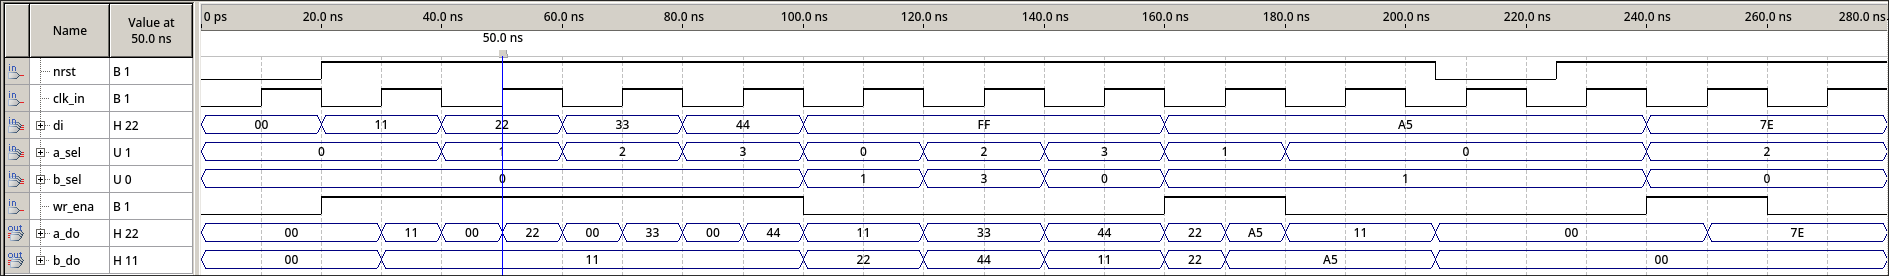
\includegraphics[width=\textwidth]{../../project/reg_bank/reg_bank_simulation.png}
  \fonte{Autoria própria (Quartus II).}
\end{figure}

{\SingleSpacing\FloatBarrier{\scriptsize\setlength{\tabcolsep}{3pt}
\begin{longtable}{rcccccccp{5.3cm}}
\caption{Casos de teste de \texttt{reg\_bank.vwf}: visão geral.}
\label{tab:caso-reg-bank}\\
\hline $t$ (ns) & \texttt{nrst} & \texttt{di} & \texttt{a\_sel} & \texttt{b\_sel} & \texttt{wr\_ena} & \texttt{a\_do} & \texttt{b\_do} & Observação \\ \hline \endfirsthead
\hline $t$ (ns) & \texttt{nrst} & \texttt{di} & \texttt{a\_sel} & \texttt{b\_sel} & \texttt{wr\_ena} & \texttt{a\_do} & \texttt{b\_do} & Observação \\ \hline \endhead
0--20 & 0 & 00h & 0 & 0 & 0 & 00h & 00h &  \\
20--40 & 1 & 11h & 0 & 0 & 1 & 11h & 11h & solta o reset; escreve 11h em R0 \\
40--60 & 1 & 22h & 1 & 0 & 1 & 22h & 11h & escreve 22h em R1 \\
60--80 & 1 & 33h & 2 & 0 & 1 & 33h & 11h & escreve 33h em R2 \\
80--100 & 1 & 44h & 3 & 0 & 1 & 44h & 11h & escreve 44h em R3 \\
100--120 & 1 & FFh & 0 & 1 & 0 & 11h & 22h & wr\_ena = 0: lê R0 e R1 (di = FFh é ignorado) \\
120--140 & 1 & FFh & 2 & 3 & 0 & 33h & 44h & lê R2 e R3 \\
140--160 & 1 & FFh & 3 & 0 & 0 & 44h & 11h & lê R3 e R0 \\
160--180 & 1 & A5h & 1 & 1 & 1 & A5h & A5h & escreve A5h em R1 (a\_sel = b\_sel = 1) \\
180--205 & 1 & A5h & 0 & 1 & 0 & 11h & A5h & lê R0 e R1 \\
205--225 & 0 & A5h & 0 & 1 & 0 & 00h & 00h & reset assíncrono no meio do ciclo (nrst = 0) \\
225--240 & 1 & A5h & 0 & 1 & 0 & 00h & 00h & solta o reset \\
240--260 & 1 & 7Eh & 2 & 0 & 1 & 7Eh & 00h & escreve 7Eh em R2 \\
260--280 & 1 & 7Eh & 2 & 0 & 0 & 7Eh & 00h & lê R2 e R0 \\
\hline
\end{longtable}}
\vspace{-0.9cm}
\fonte{Autoria própria. Saídas do fim de cada intervalo, conforme o modelo de referência e a simulação do Quartus II.}
}

%=====================================================
\chapter{Registrador de status (\texttt{reg\_status})}
\label{cap:reg_status}

\section{Especificação}

O \texttt{reg\_status} reúne cinco registradores de 1 bit independentes (RN, RV, RZ, RH e RC) para armazenar as \textit{flags} da ALU do TP1 \cite{tp2}. Cada bit de \texttt{status\_reg\_out} é atualizado na borda de subida de \texttt{clk\_in} apenas se o bit correspondente de \texttt{status\_reg\_wr\_ena} estiver em \texttt{'1'}. O \textit{reset} assíncrono (\texttt{nrst = '0'}) zera os cinco bits com prioridade, e a saída permanece continuamente ativa. A Figura~\ref{fig:bloco-reg-status} e os Quadros~\ref{quad:portas-reg-status} e \ref{qua:flags-alu} definem a interface e o mapeamento das \textit{flags}.

\begin{figure}[!htb]
\caption{Diagrama de blocos do registrador de status.}\label{fig:bloco-reg-status}
\centering
\begin{tikzpicture}[>={Stealth[length=2mm]}]
  \renewcommand{\fio}{0.8}
  \node[draw, minimum width=3.2cm, minimum height=3.2cm, font=\large\bfseries] (bloco) {reg\_status};
  \pentrada{1.2}{nrst}{}
  \pentrada{0.4}{clk\_in}{}
  \pentrada{-0.4}{status\_reg\_in[4..0]}{line width=1.2pt}
  \pentrada{-1.2}{status\_reg\_wr\_ena[4..0]}{line width=1.2pt}
  \psaida{0.0}{status\_reg\_out[4..0]}{line width=1.2pt}
\end{tikzpicture}
\fonte{Elaborada pelos autores, com base em \textcite{tp2}.}
\end{figure}

\begin{quadro}[!htb]
  \SingleSpacing
  \caption{Portas do registrador de status.}
  \label{quad:portas-reg-status}
  \centering
  \begin{tabular}{lcp{7.4cm}}
    \hline
    Porta & Direção & Descrição \\ \hline
    \texttt{nrst} & entrada & \textit{Reset} assíncrono (ativo baixo); zera os cinco registradores \\
    \texttt{clk\_in} & entrada & Clock; escrita na borda de subida \\
    \texttt{status\_reg\_in[4..0]} & entrada & Dados: [0] RN, [1] RV, [2] RZ, [3] RH, [4] RC \\
    \texttt{status\_reg\_wr\_ena[4..0]} & entrada & Habilitação individual por bit (ativa em nível alto) \\
    \texttt{status\_reg\_out[4..0]} & saída & Conteúdo dos cinco registradores \\ \hline
  \end{tabular}
  \fonte{Adaptado de \textcite{tp2}.}
\end{quadro}

\begin{quadro}[!htb]
  \SingleSpacing
  \caption{Correspondência entre as \textit{flags} da ALU e os registradores de status.}
  \label{qua:flags-alu}
  \centering
  \begin{tabular}{cll}
    \hline
    Bit & Registrador & \textit{Flag} da ALU (\texttt{flags\_out}) \\ \hline
    0 & RN & \textit{negative} (\texttt{n\_flag}) \\
    1 & RV & \textit{overflow} (\texttt{v\_flag}) \\
    2 & RZ & \textit{zero} (\texttt{z\_flag}) \\
    3 & RH & \textit{half carry/borrow} (\texttt{h\_flag}) \\
    4 & RC & \textit{carry/borrow} (\texttt{c\_flag}) \\ \hline
  \end{tabular}
  \fonte{Adaptado de \textcite{tp2}.}
\end{quadro}

\section{Implementação}

O próximo estado de cada bit é calculado concorrentemente pela expressão vetorial \texttt{(entrada AND ena) OR (estado AND NOT ena)}, implementando cinco multiplexadores 2:1 paralelos sem necessidade de múltiplos \texttt{IF}s. O \texttt{process(nrst, clk\_in)} zera o registrador de 5 bits quando \texttt{nrst = '0'} ou carrega o próximo estado na borda de subida. A Figura~\ref{fig:rtl-reg-status} mostra a síntese RTL (5 FFs \texttt{\$adff} e portas de seleção) e o Código~\ref{lst:reg-status} apresenta o VHDL.

\begin{figure}[!htb]
  \centering
  \caption{Circuito do registrador de status em nível RTL.}
  \label{fig:rtl-reg-status}
  \includegraphics[width=0.85\textwidth, height=0.32\textheight, keepaspectratio]{reg_status_rtl.pdf}
  \fonte{Elaborado a partir do site RapidRTL, com base no arquivo \texttt{project/reg\_status/reg\_status.vhd}.}
\end{figure}

\blocovhdl{Descrição VHDL do registrador de status.}{lst:reg-status}{reg_status}{reg_status.vhd}

\section{Simulação e resultados}

Foram simuladas cinco formas de onda: \texttt{reg\_status.vwf} (visão geral), \texttt{reg\_status\_escrita.vwf} (padrões alternados), \texttt{reg\_status\_enable.vwf} (habilitação bit a bit), \texttt{reg\_status\_alu.vwf} (atualização seletiva de \textit{flags} por instrução da ALU) e \texttt{reg\_status\_reset.vwf} (reset assíncrono). A Figura~\ref{fig:sim-reg-status} e a Tabela~\ref{tab:caso-reg-status} ilustram a simulação principal, demonstrando a carga total (\texttt{11111} em 30\,ns), a limpeza individual de cada bit (40--140\,ns), a escrita seletiva apenas nos bits habilitados (140--180\,ns), a retenção com \texttt{wr\_ena = 00000} e o \textit{reset} imediato em 205\,ns.

\begin{figure}[!htb]
  \centering
  \caption{Simulação funcional de \texttt{reg\_status.vwf} (visão geral).}
  \label{fig:sim-reg-status}
  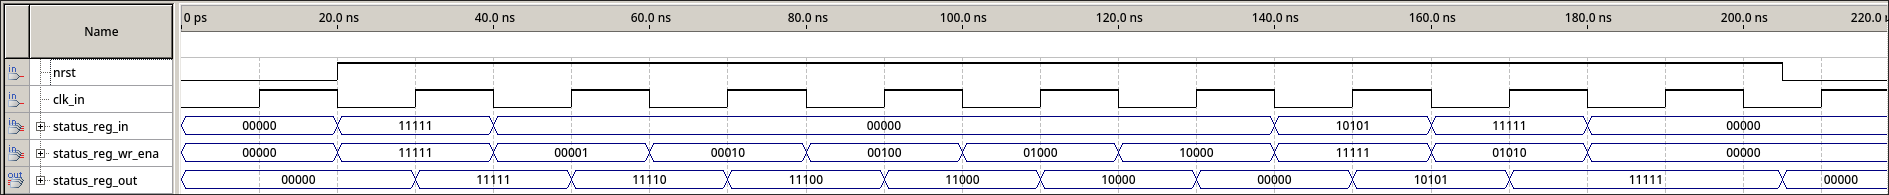
\includegraphics[width=\textwidth]{../../project/reg_status/reg_status_simulation.png}
  \fonte{Autoria própria (Quartus II).}
\end{figure}

{\SingleSpacing\FloatBarrier{\scriptsize\setlength{\tabcolsep}{3pt}
\begin{longtable}{rccccp{4.4cm}}
\caption{Casos de teste de \texttt{reg\_status.vwf}: visão geral.}
\label{tab:caso-reg-status}\\
\hline $t$ (ns) & \texttt{nrst} & \texttt{status\_reg\_in} & \texttt{status\_reg\_wr\_ena} & \texttt{status\_reg\_out} & Observação \\ \hline \endfirsthead
\hline $t$ (ns) & \texttt{nrst} & \texttt{status\_reg\_in} & \texttt{status\_reg\_wr\_ena} & \texttt{status\_reg\_out} & Observação \\ \hline \endhead
0--20 & 0 & 00000 & 00000 & 00000 &  \\
20--40 & 1 & 11111 & 11111 & 11111 & solta o reset; escreve 11111 (todos habilitados) \\
40--60 & 1 & 00000 & 00001 & 11110 & zera só RN \\
60--80 & 1 & 00000 & 00010 & 11100 & zera só RV \\
80--100 & 1 & 00000 & 00100 & 11000 & zera só RZ \\
100--120 & 1 & 00000 & 01000 & 10000 & zera só RH \\
120--140 & 1 & 00000 & 10000 & 00000 & zera só RC \\
140--160 & 1 & 10101 & 11111 & 10101 & escreve 10101 em todos \\
160--180 & 1 & 11111 & 01010 & 11111 & in = 11111, mas só RV e RH habilitados \\
180--205 & 1 & 00000 & 00000 & 11111 & ninguém habilitado: mantém \\
205--220 & 0 & 00000 & 00000 & 00000 & reset assíncrono \\
\hline
\end{longtable}}
\vspace{-0.9cm}
\fonte{Autoria própria. Saídas do fim de cada intervalo, conforme o modelo de referência e a simulação do Quartus II.}
}

%=====================================================
\chapter{Pilha (\texttt{stack})}
\label{cap:stack}

\section{Especificação}

O bloco \texttt{stack} implementa uma pilha LIFO de oito registradores de 11 bits para endereços de retorno do PC \cite{tp2}. Na borda de subida de \texttt{clk\_in}: \texttt{stack\_push = '1'} grava \texttt{stack\_in} no topo (\texttt{r(0)}) e desloca \texttt{r(0..6)} para \texttt{r(1..7)}; \texttt{stack\_pop = '1'} desloca \texttt{r(1..7)} para \texttt{r(0..6)} e insere zero em \texttt{r(7)}. O \textit{push} tem prioridade sobre o \textit{pop}, e \texttt{nrst = '0'} zera toda a pilha assincronamente com prioridade máxima. Mais de oito \textit{pushes} causam descarte do dado mais antigo (\textit{overflow}). A saída \texttt{stack\_out} expõe continuamente o topo (\texttt{r(0)}). A Figura~\ref{fig:bloco-stack} e o Quadro~\ref{quad:portas-stack} resumem o bloco.

\begin{figure}[!htb]
\caption{Diagrama de blocos da pilha.}\label{fig:bloco-stack}
\centering
\begin{tikzpicture}[>={Stealth[length=2mm]}]
  \renewcommand{\fio}{1.4}
  \node[draw, minimum width=3.0cm, minimum height=3.4cm, font=\large\bfseries] (bloco) {stack};
  \pentrada{1.3}{nrst}{}
  \pentrada{0.65}{clk\_in}{}
  \pentrada{0}{stack\_in[10..0]}{line width=1.2pt}
  \pentrada{-0.65}{stack\_push}{}
  \pentrada{-1.3}{stack\_pop}{}
  \psaida{0}{stack\_out[10..0]}{line width=1.2pt}
\end{tikzpicture}
\fonte{Elaborada pelos autores, com base em \textcite{tp2}.}
\end{figure}

\begin{quadro}[!htb]
  \SingleSpacing
  \caption{Portas da pilha.}
  \label{quad:portas-stack}
  \centering
  \begin{tabular}{lcp{9cm}}
    \hline
    Porta & Direção & Descrição \\ \hline
    \texttt{nrst} & entrada & \textit{Reset} assíncrono (ativo baixo); zera as oito posições \\
    \texttt{clk\_in} & entrada & Clock; \textit{push} e \textit{pop} na borda de subida \\
    \texttt{stack\_in[10..0]} & entrada & Endereço a ser empilhado \\
    \texttt{stack\_push} & entrada & Habilita o \textit{push} (ativo alto; prioritário sobre \textit{pop}) \\
    \texttt{stack\_pop} & entrada & Habilita o \textit{pop} (ativo alto) \\
    \texttt{stack\_out[10..0]} & saída & Topo da pilha (primeiro registrador), sempre ativo \\ \hline
  \end{tabular}
  \fonte{Adaptado de \textcite{tp2}.}
\end{quadro}

\section{Implementação}

A pilha usa um \textit{array} \texttt{r(0 TO 7)} de 11 bits atualizado em um único \texttt{process(nrst, clk\_in)}. Após o teste prioritário de \texttt{nrst = '0'}, a borda de subida avalia \texttt{IF stack\_push = '1'} antes de \texttt{ELSIF stack\_pop = '1'}, garantindo a prioridade do \textit{push} e realizando o deslocamento em linha única por atribuição de fatias (\texttt{r(1 TO 7) <= r(0 TO 6)} no \textit{push} e \texttt{r(0 TO 6) <= r(1 TO 7)} no \textit{pop}). A Figura~\ref{fig:rtl-stack} mostra o circuito RTL (registrador de 88 bits \texttt{\$adffe} habilitado por \texttt{push OR pop} e dois multiplexadores em cascata), e o Código~\ref{lst:stack} traz o código VHDL.

\begin{figure}[!htb]
  \centering
  \caption{Circuito da pilha em nível RTL.}
  \label{fig:rtl-stack}
  \includegraphics[width=\textwidth, height=0.32\textheight, keepaspectratio]{stack_rtl.pdf}
  \fonte{Elaborado a partir do site RapidRTL, com base no arquivo \texttt{project/stack/stack.vhd}.}
\end{figure}

\blocovhdl{Descrição VHDL da pilha.}{lst:stack}{stack}{stack.vhd}

\section{Simulação e resultados}

O bloco foi verificado em cinco arquivos \texttt{.vwf}: \texttt{stack.vwf} (visão geral), \texttt{stack\_lifo.vwf} (8 \textit{pushes} e 9 \textit{pops}), \texttt{stack\_overflow.vwf} (10 \textit{pushes} com perda dos 2 mais antigos), \texttt{stack\_push\_pop.vwf} (simultaneidade e pulsos entre bordas) e \texttt{stack\_reset.vwf} (reset assíncrono). A Figura~\ref{fig:sim-stack} e a Tabela~\ref{tab:caso-stack} comprovam a ordem LIFO nos \textit{pushes} (100, 200, 300) e \textit{pops} (200, 100), a prioridade do \textit{push} sobre o \textit{pop} em 150\,ns (empilhando 555 sobre 400) e o retorno a zero ao esvaziar a pilha.

\begin{figure}[!htb]
  \centering
  \caption{Simulação funcional de \texttt{stack.vwf} (visão geral).}
  \label{fig:sim-stack}
  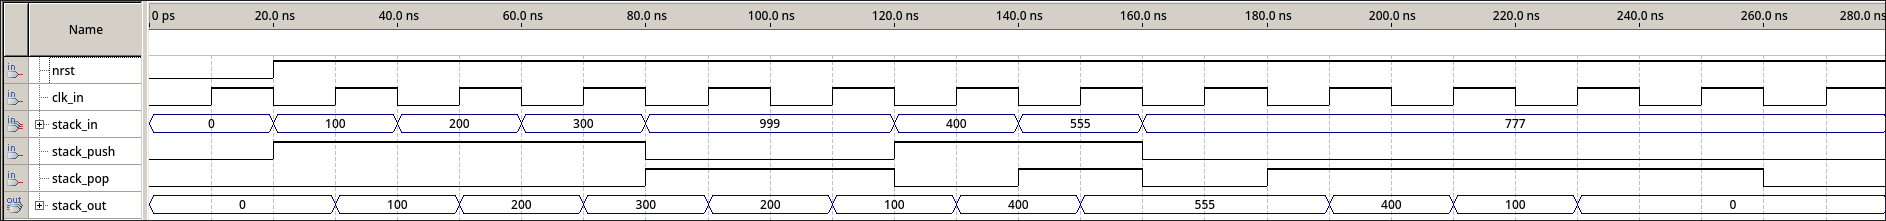
\includegraphics[width=\textwidth]{../../project/stack/stack_simulation.png}
  \fonte{Autoria própria (Quartus II).}
\end{figure}

{\SingleSpacing\FloatBarrier{\scriptsize\setlength{\tabcolsep}{3pt}
\begin{longtable}{rcccccp{5.7cm}}
\caption{Casos de teste de \texttt{stack.vwf}: visão geral.}
\label{tab:caso-stack}\\
\hline $t$ (ns) & \texttt{nrst} & \texttt{stack\_in} & \texttt{stack\_push} & \texttt{stack\_pop} & \texttt{stack\_out} & Observação \\ \hline \endfirsthead
\hline $t$ (ns) & \texttt{nrst} & \texttt{stack\_in} & \texttt{stack\_push} & \texttt{stack\_pop} & \texttt{stack\_out} & Observação \\ \hline \endhead
0--20 & 0 & 0 & 0 & 0 & 0 &  \\
20--40 & 1 & 100 & 1 & 0 & 100 & solta o reset; push 100 \\
40--60 & 1 & 200 & 1 & 0 & 200 & push 200 \\
60--80 & 1 & 300 & 1 & 0 & 300 & push 300 \\
80--100 & 1 & 999 & 0 & 1 & 200 & pop (volta a 200) \\
100--120 & 1 & 999 & 0 & 1 & 100 & pop (volta a 100) \\
120--140 & 1 & 400 & 1 & 0 & 400 & push 400 \\
140--160 & 1 & 555 & 1 & 1 & 555 & push e pop juntos: push 555 vence \\
160--180 & 1 & 777 & 0 & 0 & 555 & sem operação (stack\_in muda e é ignorado) \\
180--200 & 1 & 777 & 0 & 1 & 400 & pop (555 sai, volta a 400) \\
200--220 & 1 & 777 & 0 & 1 & 100 & pop (volta a 100) \\
220--240 & 1 & 777 & 0 & 1 & 0 & pop (esvazia, topo = 0) \\
240--260 & 1 & 777 & 0 & 1 & 0 & pop com a pilha vazia: continua 0 \\
260--280 & 1 & 777 & 0 & 0 & 0 & sem operação \\
\hline
\end{longtable}}
\vspace{-0.9cm}
\fonte{Autoria própria. Saídas do fim de cada intervalo, conforme o modelo de referência e a simulação do Quartus II.}
}

%=====================================================
\chapter{Contador de programa (\texttt{prog\_cnt})}
\label{cap:prog_cnt}

\section{Especificação}

O \texttt{prog\_cnt} é um contador síncrono de 11 bits (módulo 2048, de 0 a 2047) com \textit{reset} assíncrono prioritário (\texttt{nrst = '0'}) \cite{tp2}. Fornece o valor atual registrado (\texttt{pc\_out}) e o próximo valor combinacional (\texttt{next\_pc\_out}), selecionado por \texttt{pc\_ctrl} conforme o Quadro~\ref{quad:pc-ctrl}. A Figura~\ref{fig:bloco-prog-cnt} e o Quadro~\ref{quad:portas-prog-cnt} detalham suas portas.

\begin{quadro}[!htb]
  \SingleSpacing
  \caption{Funções do contador de programa, selecionadas por \texttt{pc\_ctrl}.}
  \label{quad:pc-ctrl}
  \centering
  \begin{tabular}{cl}
    \hline
    \texttt{pc\_ctrl} & Função \\ \hline
    \texttt{00} & Permanece como está \\
    \texttt{01} & Carrega o topo da pilha (entrada \texttt{from\_stack}) \\
    \texttt{10} & Carrega um novo valor (entrada \texttt{new\_pc\_in}) \\
    \texttt{11} & Incrementa o contador ($+1$) \\ \hline
  \end{tabular}
  \fonte{Adaptado de \textcite{tp2}.}
\end{quadro}

\begin{figure}[!htb]
\caption{Diagrama de blocos do contador de programa.}\label{fig:bloco-prog-cnt}
\centering
\begin{tikzpicture}[>={Stealth[length=2mm]}]
  \renewcommand{\fio}{1.0}
  \node[draw, minimum width=3.0cm, minimum height=3.8cm, font=\large\bfseries] (bloco) {prog\_cnt};
  \pentrada{1.5}{nrst}{}
  \pentrada{0.8}{clk\_in}{}
  \pentrada{0.1}{pc\_ctrl[1..0]}{line width=1.2pt}
  \pentrada{-0.6}{new\_pc\_in[10..0]}{line width=1.2pt}
  \pentrada{-1.3}{from\_stack[10..0]}{line width=1.2pt}
  \psaida{0.6}{next\_pc\_out[10..0]}{line width=1.2pt}
  \psaida{-0.6}{pc\_out[10..0]}{line width=1.2pt}
\end{tikzpicture}
\fonte{Elaborada pelos autores, com base em \textcite{tp2}.}
\end{figure}

\begin{quadro}[!htb]
  \SingleSpacing
  \caption{Portas do contador de programa.}
  \label{quad:portas-prog-cnt}
  \centering
  \begin{tabular}{lcp{8.8cm}}
    \hline
    Porta & Direção & Descrição \\ \hline
    \texttt{nrst} & entrada & \textit{Reset} assíncrono (ativo baixo); zera o contador \\
    \texttt{clk\_in} & entrada & Clock; incremento e carga na borda de subida \\
    \texttt{pc\_ctrl[1..0]} & entrada & Seleção de função (Quadro~\ref{quad:pc-ctrl}) \\
    \texttt{new\_pc\_in[10..0]} & entrada & Valor carregado quando \texttt{pc\_ctrl = "10"} \\
    \texttt{from\_stack[10..0]} & entrada & Valor carregado quando \texttt{pc\_ctrl = "01"} \\
    \texttt{next\_pc\_out[10..0]} & saída & Próximo valor do contador (saída combinacional) \\
    \texttt{pc\_out[10..0]} & saída & Valor atual do contador (saída dos \textit{flip-flops}) \\ \hline
  \end{tabular}
  \fonte{Adaptado de \textcite{tp2}.}
\end{quadro}

\section{Implementação}

O circuito separa a lógica de próximo estado e o registrador: um comando concorrente \texttt{WITH pc\_ctrl SELECT} define \texttt{next\_pc} entre \texttt{pc}, \texttt{from\_stack}, \texttt{new\_pc\_in} e \texttt{pc + 1} (cuja soma em 11 bits com \texttt{std\_logic\_unsigned} realiza naturalmente a contagem módulo 2048), enquanto o \texttt{process(nrst, clk\_in)} zera \texttt{pc} no reset ou registra \texttt{pc <= next\_pc} na borda de subida. A Figura~\ref{fig:rtl-prog-cnt} apresenta o circuito RTL e o Código~\ref{lst:prog-cnt}, a descrição VHDL.

\begin{figure}[!htb]
  \centering
  \caption{Circuito do contador de programa em nível RTL.}
  \label{fig:rtl-prog-cnt}
  \includegraphics[width=0.55\textwidth, height=0.38\textheight, keepaspectratio]{prog_cnt_rtl.pdf}
  \fonte{Elaborado a partir do site RapidRTL, com base no arquivo \texttt{project/prog\_cnt/prog\_cnt.vhd}.}
\end{figure}

\blocovhdl{Descrição VHDL do contador de programa.}{lst:prog-cnt}{prog_cnt}{prog_cnt.vhd}

\section{Simulação e resultados}

Foram criadas quatro formas de onda: \texttt{prog\_cnt.vwf} (visão geral), \texttt{prog\_cnt\_incremento.vwf} (volta de 2047 a 0), \texttt{prog\_cnt\_carga.vwf} (cargas síncronas e resposta imediata de \texttt{next\_pc\_out}) e \texttt{prog\_cnt\_reset.vwf} (prioridade do reset). A Figura~\ref{fig:sim-prog-cnt} e a Tabela~\ref{tab:caso-prog-cnt} evidenciam o avanço de \texttt{next\_pc\_out} antes da borda e a atualização síncrona de \texttt{pc\_out} no incremento (20--80\,ns), na retenção (80--100\,ns), nas cargas de \texttt{new\_pc\_in} (100) e \texttt{from\_stack} (677) e no \textit{reset} assíncrono em 205\,ns.

\begin{figure}[!htb]
  \centering
  \caption{Simulação funcional de \texttt{prog\_cnt.vwf} (visão geral).}
  \label{fig:sim-prog-cnt}
  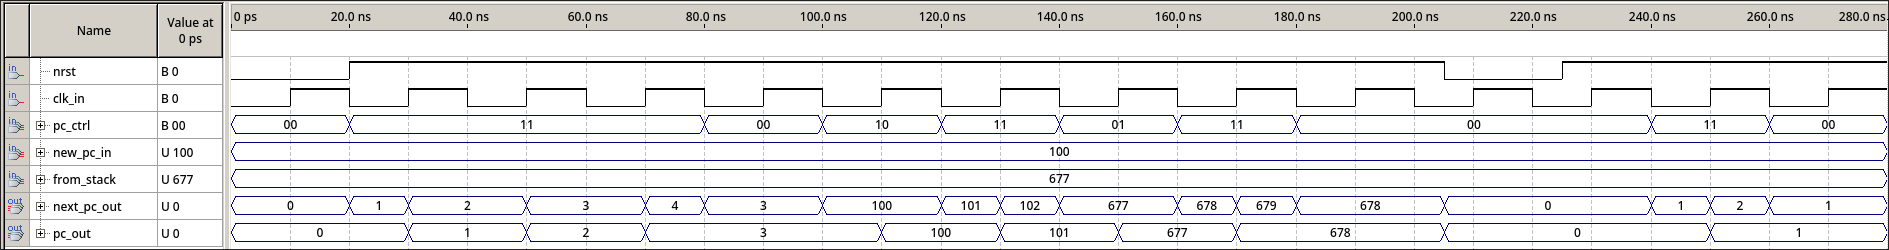
\includegraphics[width=\textwidth]{../../project/prog_cnt/prog_cnt_simulation.png}
  \fonte{Autoria própria (Quartus II).}
\end{figure}

{\SingleSpacing\FloatBarrier{\scriptsize\setlength{\tabcolsep}{3pt}
\begin{longtable}{rccccccp{4.2cm}}
\caption{Casos de teste de \texttt{prog\_cnt.vwf}: visão geral.}
\label{tab:caso-prog-cnt}\\
\hline $t$ (ns) & \texttt{nrst} & \texttt{pc\_ctrl} & \texttt{new\_pc\_in} & \texttt{from\_stack} & \texttt{next\_pc\_out} & \texttt{pc\_out} & Observação \\ \hline \endfirsthead
\hline $t$ (ns) & \texttt{nrst} & \texttt{pc\_ctrl} & \texttt{new\_pc\_in} & \texttt{from\_stack} & \texttt{next\_pc\_out} & \texttt{pc\_out} & Observação \\ \hline \endhead
0--20 & 0 & 00 & 100 & 677 & 0 & 0 &  \\
20--40 & 1 & 11 & 100 & 677 & 2 & 1 & solta o reset; incrementa \\
40--60 & 1 & 11 & 100 & 677 & 3 & 2 & incrementa \\
60--80 & 1 & 11 & 100 & 677 & 4 & 3 & incrementa \\
80--100 & 1 & 00 & 100 & 677 & 3 & 3 & mantém (00) \\
100--120 & 1 & 10 & 100 & 677 & 100 & 100 & carrega new\_pc\_in = 100 \\
120--140 & 1 & 11 & 100 & 677 & 102 & 101 & incrementa \\
140--160 & 1 & 01 & 100 & 677 & 677 & 677 & carrega from\_stack = 677 \\
160--180 & 1 & 11 & 100 & 677 & 679 & 678 & incrementa \\
180--205 & 1 & 00 & 100 & 677 & 678 & 678 & mantém \\
205--225 & 0 & 00 & 100 & 677 & 0 & 0 & reset assíncrono \\
225--240 & 1 & 00 & 100 & 677 & 0 & 0 & solta o reset \\
240--260 & 1 & 11 & 100 & 677 & 2 & 1 & incrementa \\
260--280 & 1 & 00 & 100 & 677 & 1 & 1 & mantém \\
\hline
\end{longtable}}
\vspace{-0.9cm}
\fonte{Autoria própria. Saídas do fim de cada intervalo, conforme o modelo de referência e a simulação do Quartus II.}
}

%=====================================================
\chapter{Conclusão}
\label{cap:conclusao}

Os quatro módulos sequenciais especificados (\texttt{reg\_bank}, \texttt{reg\_status}, \texttt{stack} e \texttt{prog\_cnt}) foram implementados em VHDL e validados com sucesso. A separação entre lógica combinacional concorrente e processos restritos aos registradores sensíveis a \texttt{nrst} e \texttt{clk\_in} eliminou a inferência de \textit{latches} indesejados e resultou exatamente na contagem esperada de \textit{flip-flops} ($32$, $5$, $88$ e $11$). O Quadro~\ref{quad:recursos} sintetiza o uso de recursos e a frequência máxima no Cyclone II EP2C35F672C6, confirmando operação folgada acima dos 50\,MHz da placa DE2. Todas as simulações funcionais no Quartus II concordaram integralmente com os valores esperados, deixando os blocos prontos para integração com a ALU (TP1) e com a unidade de controle nos próximos trabalhos.

\begin{quadro}[!htb]
  \SingleSpacing
  \caption{Recursos e \textit{timing} de cada bloco no Cyclone II EP2C35F672C6, com clock de 50\,MHz.}
  \label{quad:recursos}
  \centering
  \begin{tabular}{lcccc}
    \hline
    Bloco & Elementos lógicos & \textit{Flip-flops} & Pinos & $f_{max}$ (modelo lento) \\ \hline
    \texttt{reg\_bank}   & 36 & 32 & 31 & 78,9\,MHz \\
    \texttt{reg\_status} & 5  & 5  & 17 & 125,8\,MHz \\
    \texttt{stack}       & 89 & 88 & 26 & 125,6\,MHz \\
    \texttt{prog\_cnt}   & 33 & 11 & 48 & 65,6\,MHz \\ \hline
  \end{tabular}
  \fonte{Relatórios de compilação do Quartus II (\textit{Fitter} e TimeQuest).}
\end{quadro}

% ELEMENTOS PÓS-TEXTUAIS ------------------------------------------------------
\postextual
\pagestyle{plain}

{\SingleSpacing
\printbibliography[heading=bibintoc,title={Referências}]
}

\begin{apendicesenv}
\chapter{Arquivos do projeto}
\label{ap:arquivos}

Cada bloco possui um projeto independente em \texttt{project/<nome>/} (\texttt{reg\_bank}, \texttt{reg\_status}, \texttt{stack} e \texttt{prog\_cnt}) contendo:
\begin{description}
  \item[\texttt{<nome>.vhd}, \texttt{.qpf}, \texttt{.qsf}, \texttt{.sdc}] código VHDL, projeto Quartus II para o Cyclone II EP2C35F672C6 e restrição temporal de 50\,MHz;
  \item[\texttt{<nome>*.vwf} e \texttt{<nome>\_simulation.png}] arquivos de estímulo de simulação e captura da forma de onda principal;
  \item[\texttt{<nome>\_rtl.svg}] esquemático RTL extraído via RapidRTL e convertido em PDF pelo \texttt{.justfile}.
\end{description}

\chapter{Casos de teste das demais formas de onda}
\label{ap:tabelas}

Apresentam-se a seguir as tabelas de valores esperados (ao final de cada intervalo) das demais formas de onda simuladas para cada bloco.

{\SingleSpacing\renewcommand{\arraystretch}{0.92}
\section{Banco de registradores}
{\scriptsize\setlength{\tabcolsep}{3pt}
\begin{longtable}{rcccccccp{5.3cm}}
\caption{Casos de teste de \texttt{reg\_bank\_escrita.vwf}: escrita nos quatro registradores.}
\label{tab:caso-reg-bank-escrita}\\
\hline $t$ (ns) & \texttt{nrst} & \texttt{di} & \texttt{a\_sel} & \texttt{b\_sel} & \texttt{wr\_ena} & \texttt{a\_do} & \texttt{b\_do} & Observação \\ \hline \endfirsthead
\hline $t$ (ns) & \texttt{nrst} & \texttt{di} & \texttt{a\_sel} & \texttt{b\_sel} & \texttt{wr\_ena} & \texttt{a\_do} & \texttt{b\_do} & Observação \\ \hline \endhead
0--20 & 0 & 00h & 0 & 0 & 0 & 00h & 00h &  \\
20--40 & 1 & A5h & 0 & 0 & 1 & A5h & A5h & escreve A5h em R0 (b\_sel = a\_sel) \\
40--60 & 1 & 5Ah & 1 & 1 & 1 & 5Ah & 5Ah & escreve 5Ah em R1 \\
60--80 & 1 & FFh & 2 & 2 & 1 & FFh & FFh & escreve FFh em R2 \\
80--100 & 1 & 01h & 3 & 3 & 1 & 01h & 01h & escreve 01h em R3 \\
100--120 & 1 & 00h & 0 & 3 & 0 & A5h & 01h & desabilita a escrita; a\_do = R0, b\_do = R3 \\
120--140 & 1 & 00h & 1 & 2 & 0 & 5Ah & FFh & a\_do = R1, b\_do = R2 \\
140--160 & 1 & 00h & 2 & 1 & 0 & FFh & 5Ah & a\_do = R2, b\_do = R1 \\
160--180 & 1 & 00h & 3 & 0 & 0 & 01h & A5h & a\_do = R3, b\_do = R0 \\
180--200 & 1 & 00h & 0 & 0 & 1 & 00h & 00h & sobrescreve R0 com 00h \\
200--220 & 1 & FFh & 3 & 3 & 1 & FFh & FFh & sobrescreve R3 com FFh \\
220--240 & 1 & FFh & 0 & 3 & 0 & 00h & FFh & lê R0 e R3 \\
240--260 & 1 & FFh & 1 & 2 & 0 & 5Ah & FFh & a\_do = R1, b\_do = R2 (intactos) \\
\hline
\end{longtable}}
\vspace{-0.9cm}
\fonte{Autoria própria. Saídas do fim de cada intervalo, conforme o modelo de referência e a simulação do Quartus II.}

{\scriptsize\setlength{\tabcolsep}{3pt}
\begin{longtable}{rcccccccp{5.3cm}}
\caption{Casos de teste de \texttt{reg\_bank\_leitura.vwf}: leitura assíncrona.}
\label{tab:caso-reg-bank-leitura}\\
\hline $t$ (ns) & \texttt{nrst} & \texttt{di} & \texttt{a\_sel} & \texttt{b\_sel} & \texttt{wr\_ena} & \texttt{a\_do} & \texttt{b\_do} & Observação \\ \hline \endfirsthead
\hline $t$ (ns) & \texttt{nrst} & \texttt{di} & \texttt{a\_sel} & \texttt{b\_sel} & \texttt{wr\_ena} & \texttt{a\_do} & \texttt{b\_do} & Observação \\ \hline \endhead
0--20 & 0 & 00h & 0 & 0 & 0 & 00h & 00h &  \\
20--40 & 1 & 10h & 0 & 0 & 1 & 10h & 10h & R0 = 10h \\
40--60 & 1 & 20h & 1 & 0 & 1 & 20h & 10h & R1 = 20h \\
60--80 & 1 & 40h & 2 & 0 & 1 & 40h & 10h & R2 = 40h \\
80--100 & 1 & 80h & 3 & 0 & 1 & 80h & 10h & R3 = 80h \\
100--105 & 1 & FFh & 3 & 0 & 0 & 80h & 10h & wr\_ena = 0, di = FFh (ignorado) \\
105--125 & 1 & FFh & 0 & 0 & 0 & 10h & 10h & a\_sel = 0, b\_sel = 0 \\
125--145 & 1 & FFh & 0 & 1 & 0 & 10h & 20h & a\_sel = 0, b\_sel = 1 \\
145--165 & 1 & FFh & 0 & 2 & 0 & 10h & 40h & a\_sel = 0, b\_sel = 2 \\
165--185 & 1 & FFh & 0 & 3 & 0 & 10h & 80h & a\_sel = 0, b\_sel = 3 \\
185--205 & 1 & FFh & 1 & 0 & 0 & 20h & 10h & a\_sel = 1, b\_sel = 0 \\
205--225 & 1 & FFh & 1 & 1 & 0 & 20h & 20h & a\_sel = 1, b\_sel = 1 \\
225--245 & 1 & FFh & 1 & 2 & 0 & 20h & 40h & a\_sel = 1, b\_sel = 2 \\
245--265 & 1 & FFh & 1 & 3 & 0 & 20h & 80h & a\_sel = 1, b\_sel = 3 \\
265--285 & 1 & FFh & 2 & 0 & 0 & 40h & 10h & a\_sel = 2, b\_sel = 0 \\
285--305 & 1 & FFh & 2 & 1 & 0 & 40h & 20h & a\_sel = 2, b\_sel = 1 \\
305--325 & 1 & FFh & 2 & 2 & 0 & 40h & 40h & a\_sel = 2, b\_sel = 2 \\
325--345 & 1 & FFh & 2 & 3 & 0 & 40h & 80h & a\_sel = 2, b\_sel = 3 \\
345--365 & 1 & FFh & 3 & 0 & 0 & 80h & 10h & a\_sel = 3, b\_sel = 0 \\
365--385 & 1 & FFh & 3 & 1 & 0 & 80h & 20h & a\_sel = 3, b\_sel = 1 \\
385--405 & 1 & FFh & 3 & 2 & 0 & 80h & 40h & a\_sel = 3, b\_sel = 2 \\
405--420 & 1 & FFh & 3 & 3 & 0 & 80h & 80h & a\_sel = 3, b\_sel = 3 \\
\hline
\end{longtable}}
\vspace{-0.9cm}
\fonte{Autoria própria. Saídas do fim de cada intervalo, conforme o modelo de referência e a simulação do Quartus II.}

{\scriptsize\setlength{\tabcolsep}{3pt}
\begin{longtable}{rcccccccp{5.3cm}}
\caption{Casos de teste de \texttt{reg\_bank\_wr\_ena.vwf}: habilitação da escrita.}
\label{tab:caso-reg-bank-wr-ena}\\
\hline $t$ (ns) & \texttt{nrst} & \texttt{di} & \texttt{a\_sel} & \texttt{b\_sel} & \texttt{wr\_ena} & \texttt{a\_do} & \texttt{b\_do} & Observação \\ \hline \endfirsthead
\hline $t$ (ns) & \texttt{nrst} & \texttt{di} & \texttt{a\_sel} & \texttt{b\_sel} & \texttt{wr\_ena} & \texttt{a\_do} & \texttt{b\_do} & Observação \\ \hline \endhead
0--20 & 0 & 00h & 0 & 0 & 0 & 00h & 00h &  \\
20--40 & 1 & 11h & 0 & 0 & 1 & 11h & 11h & escreve 11h em R0 \\
40--60 & 1 & 99h & 0 & 0 & 0 & 11h & 11h & wr\_ena = 0, di = 99h: R0 não muda \\
60--80 & 1 & 88h & 0 & 0 & 0 & 11h & 11h & di = 88h: R0 continua 11h \\
80--100 & 1 & 99h & 0 & 0 & 1 & 99h & 99h & wr\_ena = 1: escreve 99h em R0 \\
100--120 & 1 & 00h & 0 & 0 & 0 & 99h & 99h & wr\_ena = 0 \\
120--132 & 1 & 66h & 1 & 1 & 0 & 00h & 00h & prepara R1 = 66h, mas sem escrever \\
132--138 & 1 & 66h & 1 & 1 & 1 & 00h & 00h & pulso de wr\_ena entre duas bordas (12 a 18 ns): não escreve \\
138--148 & 1 & 66h & 1 & 1 & 0 & 00h & 00h & fim do pulso \\
148--152 & 1 & 66h & 1 & 1 & 1 & 66h & 66h & pulso de wr\_ena sobre a borda de subida (8 a 12 ns): escreve 66h em R1 \\
152--160 & 1 & 66h & 1 & 1 & 0 & 66h & 66h & fim do pulso \\
160--180 & 1 & 66h & 1 & 0 & 0 & 66h & 99h & lê R1 e R0 \\
180--200 & 1 & 66h & 0 & 1 & 0 & 99h & 66h & lê R0 e R1 \\
\hline
\end{longtable}}
\vspace{-0.9cm}
\fonte{Autoria própria. Saídas do fim de cada intervalo, conforme o modelo de referência e a simulação do Quartus II.}

{\scriptsize\setlength{\tabcolsep}{3pt}
\begin{longtable}{rcccccccp{5.3cm}}
\caption{Casos de teste de \texttt{reg\_bank\_reset.vwf}: reset assíncrono.}
\label{tab:caso-reg-bank-reset}\\
\hline $t$ (ns) & \texttt{nrst} & \texttt{di} & \texttt{a\_sel} & \texttt{b\_sel} & \texttt{wr\_ena} & \texttt{a\_do} & \texttt{b\_do} & Observação \\ \hline \endfirsthead
\hline $t$ (ns) & \texttt{nrst} & \texttt{di} & \texttt{a\_sel} & \texttt{b\_sel} & \texttt{wr\_ena} & \texttt{a\_do} & \texttt{b\_do} & Observação \\ \hline \endhead
0--20 & 0 & 00h & 0 & 0 & 0 & 00h & 00h &  \\
20--40 & 1 & C1h & 0 & 0 & 1 & C1h & C1h & escreve C1h em R0 \\
40--60 & 1 & C2h & 1 & 0 & 1 & C2h & C1h & escreve C2h em R1 \\
60--80 & 1 & C3h & 2 & 0 & 1 & C3h & C1h & escreve C3h em R2 \\
80--85 & 1 & C3h & 0 & 1 & 0 & C1h & C2h & a\_do = R0, b\_do = R1; wr\_ena = 0 \\
85--100 & 0 & C3h & 0 & 1 & 0 & 00h & 00h & reset assíncrono (fora de qualquer borda): tudo vai a 0 \\
100--123 & 0 & EEh & 1 & 1 & 1 & 00h & 00h & ainda em reset; wr\_ena = 1 sobre a borda: não escreve \\
123--140 & 1 & EEh & 1 & 1 & 1 & EEh & EEh & solta o reset (a borda em 130 ns já pode escrever) \\
140--160 & 1 & EEh & 0 & 1 & 0 & 00h & EEh & wr\_ena = 0 \\
160--180 & 1 & D1h & 0 & 1 & 1 & D1h & EEh & escreve D1h em R0 \\
180--212 & 1 & D1h & 0 & 1 & 0 & D1h & EEh & wr\_ena = 0 \\
212--215 & 0 & D1h & 0 & 1 & 0 & 00h & 00h & pulso de reset de 3 ns, sem borda: ainda zera \\
215--220 & 1 & D1h & 0 & 1 & 0 & 00h & 00h & fim do pulso \\
220--240 & 1 & D1h & 0 & 1 & 0 & 00h & 00h & tudo em 0 \\
\hline
\end{longtable}}
\vspace{-0.9cm}
\fonte{Autoria própria. Saídas do fim de cada intervalo, conforme o modelo de referência e a simulação do Quartus II.}


\section{Registrador de status}
{\scriptsize\setlength{\tabcolsep}{3pt}
\begin{longtable}{rccccp{4.4cm}}
\caption{Casos de teste de \texttt{reg\_status\_escrita.vwf}: escrita de todos os bits.}
\label{tab:caso-reg-status-escrita}\\
\hline $t$ (ns) & \texttt{nrst} & \texttt{status\_reg\_in} & \texttt{status\_reg\_wr\_ena} & \texttt{status\_reg\_out} & Observação \\ \hline \endfirsthead
\hline $t$ (ns) & \texttt{nrst} & \texttt{status\_reg\_in} & \texttt{status\_reg\_wr\_ena} & \texttt{status\_reg\_out} & Observação \\ \hline \endhead
0--20 & 0 & 00000 & 00000 & 00000 &  \\
20--40 & 1 & 10101 & 11111 & 10101 & escreve 10101 \\
40--60 & 1 & 01010 & 11111 & 01010 & escreve 01010 \\
60--80 & 1 & 11111 & 11111 & 11111 & escreve 11111 \\
80--100 & 1 & 00000 & 11111 & 00000 & escreve 00000 \\
100--120 & 1 & 11111 & 11111 & 11111 & escreve 11111 \\
120--140 & 1 & 00110 & 11111 & 00110 & escreve 00110 \\
140--160 & 1 & 11001 & 00000 & 00110 & mantém 00110 (clock continua) \\
\hline
\end{longtable}}
\vspace{-0.9cm}
\fonte{Autoria própria. Saídas do fim de cada intervalo, conforme o modelo de referência e a simulação do Quartus II.}

{\scriptsize\setlength{\tabcolsep}{3pt}
\begin{longtable}{rccccp{4.4cm}}
\caption{Casos de teste de \texttt{reg\_status\_enable.vwf}: habilitação bit a bit.}
\label{tab:caso-reg-status-enable}\\
\hline $t$ (ns) & \texttt{nrst} & \texttt{status\_reg\_in} & \texttt{status\_reg\_wr\_ena} & \texttt{status\_reg\_out} & Observação \\ \hline \endfirsthead
\hline $t$ (ns) & \texttt{nrst} & \texttt{status\_reg\_in} & \texttt{status\_reg\_wr\_ena} & \texttt{status\_reg\_out} & Observação \\ \hline \endhead
0--20 & 0 & 00000 & 00000 & 00000 &  \\
20--40 & 1 & 11111 & 00001 & 00001 & seta só RN \\
40--60 & 1 & 11111 & 00010 & 00011 & seta só RV \\
60--80 & 1 & 11111 & 00100 & 00111 & seta só RZ \\
80--100 & 1 & 11111 & 01000 & 01111 & seta só RH \\
100--120 & 1 & 11111 & 10000 & 11111 & seta só RC \\
120--140 & 1 & 00000 & 00000 & 11111 & ninguém habilitado, in = 00000: mantém 11111 \\
140--160 & 1 & 00000 & 00001 & 11110 & zera só RN \\
160--180 & 1 & 00000 & 00010 & 11100 & zera só RV \\
180--200 & 1 & 00000 & 00100 & 11000 & zera só RZ \\
200--220 & 1 & 00000 & 01000 & 10000 & zera só RH \\
220--240 & 1 & 00000 & 10000 & 00000 & zera só RC \\
240--260 & 1 & 10101 & 10101 & 10101 & habilita RN, RZ, RC com in = 10101 \\
260--280 & 1 & 01010 & 11010 & 01111 & habilita os outros dois com in = 01010 e RC com 0 \\
\hline
\end{longtable}}
\vspace{-0.9cm}
\fonte{Autoria própria. Saídas do fim de cada intervalo, conforme o modelo de referência e a simulação do Quartus II.}

{\scriptsize\setlength{\tabcolsep}{3pt}
\begin{longtable}{rccccp{4.4cm}}
\caption{Casos de teste de \texttt{reg\_status\_alu.vwf}: uso com a ALU (flags C H Z V N).}
\label{tab:caso-reg-status-alu}\\
\hline $t$ (ns) & \texttt{nrst} & \texttt{status\_reg\_in} & \texttt{status\_reg\_wr\_ena} & \texttt{status\_reg\_out} & Observação \\ \hline \endfirsthead
\hline $t$ (ns) & \texttt{nrst} & \texttt{status\_reg\_in} & \texttt{status\_reg\_wr\_ena} & \texttt{status\_reg\_out} & Observação \\ \hline \endhead
0--20 & 0 & 00000 & 00000 & 00000 &  \\
20--40 & 1 & 11100 & 11111 & 11100 & ADD 77h+89h = 00h: C=1 H=1 Z=1 V=0 N=0, todos habilitados \\
40--60 & 1 & 00000 & 00101 & 11000 & AND resultado 30h: só N=0 e Z=0 são atualizados (C, H, V preservados) \\
60--80 & 1 & 01010 & 11111 & 01010 & SUB 80h-01h = 7Fh: C=0 H=1 Z=0 V=1 N=0, todos habilitados \\
80--100 & 1 & 00100 & 00101 & 01110 & XOR resultado 00h: só N=0 e Z=1 \\
100--120 & 1 & 10001 & 10101 & 11011 & SRA 81h = C0h: C=1 Z=0 N=1 (H e V preservados) \\
120--140 & 1 & 11111 & 00000 & 11011 & nenhum flag atualizado (instrução que não altera flags) \\
140--160 & 1 & 00000 & 11111 & 00000 & ADD 01h+01h = 02h: tudo 0 \\
160--180 & 1 & 10001 & 11111 & 10001 & ADD C7h+D0h = 97h: C=1 H=0 Z=0 V=0 N=1 \\
180--200 & 1 & 10001 & 11111 & 10001 & mantém \\
\hline
\end{longtable}}
\vspace{-0.9cm}
\fonte{Autoria própria. Saídas do fim de cada intervalo, conforme o modelo de referência e a simulação do Quartus II.}

{\scriptsize\setlength{\tabcolsep}{3pt}
\begin{longtable}{rccccp{4.4cm}}
\caption{Casos de teste de \texttt{reg\_status\_reset.vwf}: reset assíncrono.}
\label{tab:caso-reg-status-reset}\\
\hline $t$ (ns) & \texttt{nrst} & \texttt{status\_reg\_in} & \texttt{status\_reg\_wr\_ena} & \texttt{status\_reg\_out} & Observação \\ \hline \endfirsthead
\hline $t$ (ns) & \texttt{nrst} & \texttt{status\_reg\_in} & \texttt{status\_reg\_wr\_ena} & \texttt{status\_reg\_out} & Observação \\ \hline \endhead
0--20 & 0 & 00000 & 00000 & 00000 &  \\
20--40 & 1 & 11111 & 11111 & 11111 & escreve 11111 \\
40--65 & 1 & 11111 & 00000 & 11111 & mantém \\
65--80 & 0 & 11111 & 00000 & 00000 & reset assíncrono, fora de qualquer borda \\
80--103 & 0 & 11111 & 11111 & 00000 & ainda em reset; escrita habilitada sobre a borda: não escreve \\
103--120 & 1 & 11111 & 11111 & 11111 & solta o reset \\
120--140 & 1 & 10101 & 11111 & 10101 & escreve 10101 (a borda desse ciclo já escreve) \\
140--172 & 1 & 10101 & 00000 & 10101 & mantém \\
172--175 & 0 & 10101 & 00000 & 00000 & pulso de reset de 3 ns, sem borda \\
175--180 & 1 & 10101 & 00000 & 00000 & fim do pulso \\
180--200 & 1 & 10101 & 00000 & 00000 & tudo em 0 \\
\hline
\end{longtable}}
\vspace{-0.9cm}
\fonte{Autoria própria. Saídas do fim de cada intervalo, conforme o modelo de referência e a simulação do Quartus II.}


\section{Pilha}
{\scriptsize\setlength{\tabcolsep}{3pt}
\begin{longtable}{rcccccp{5.7cm}}
\caption{Casos de teste de \texttt{stack\_lifo.vwf}: ordem LIFO.}
\label{tab:caso-stack-lifo}\\
\hline $t$ (ns) & \texttt{nrst} & \texttt{stack\_in} & \texttt{stack\_push} & \texttt{stack\_pop} & \texttt{stack\_out} & Observação \\ \hline \endfirsthead
\hline $t$ (ns) & \texttt{nrst} & \texttt{stack\_in} & \texttt{stack\_push} & \texttt{stack\_pop} & \texttt{stack\_out} & Observação \\ \hline \endhead
0--20 & 0 & 0 & 0 & 0 & 0 &  \\
20--40 & 1 & 100 & 1 & 0 & 100 & push 100 \\
40--60 & 1 & 200 & 1 & 0 & 200 & push 200 \\
60--80 & 1 & 300 & 1 & 0 & 300 & push 300 \\
80--100 & 1 & 400 & 1 & 0 & 400 & push 400 \\
100--120 & 1 & 500 & 1 & 0 & 500 & push 500 \\
120--140 & 1 & 600 & 1 & 0 & 600 & push 600 \\
140--160 & 1 & 700 & 1 & 0 & 700 & push 700 \\
160--180 & 1 & 800 & 1 & 0 & 800 & push 800 \\
180--200 & 1 & 0 & 0 & 1 & 700 & pop \\
200--220 & 1 & 0 & 0 & 1 & 600 & pop \\
220--240 & 1 & 0 & 0 & 1 & 500 & pop \\
240--260 & 1 & 0 & 0 & 1 & 400 & pop \\
260--280 & 1 & 0 & 0 & 1 & 300 & pop \\
280--300 & 1 & 0 & 0 & 1 & 200 & pop \\
300--320 & 1 & 0 & 0 & 1 & 100 & pop \\
320--340 & 1 & 0 & 0 & 1 & 0 & pop \\
340--360 & 1 & 0 & 0 & 1 & 0 & pop extra: pilha vazia \\
360--380 & 1 & 0 & 0 & 0 & 0 & sem operação \\
\hline
\end{longtable}}
\vspace{-0.9cm}
\fonte{Autoria própria. Saídas do fim de cada intervalo, conforme o modelo de referência e a simulação do Quartus II.}

{\scriptsize\setlength{\tabcolsep}{3pt}
\begin{longtable}{rcccccp{5.7cm}}
\caption{Casos de teste de \texttt{stack\_overflow.vwf}: stack overflow.}
\label{tab:caso-stack-overflow}\\
\hline $t$ (ns) & \texttt{nrst} & \texttt{stack\_in} & \texttt{stack\_push} & \texttt{stack\_pop} & \texttt{stack\_out} & Observação \\ \hline \endfirsthead
\hline $t$ (ns) & \texttt{nrst} & \texttt{stack\_in} & \texttt{stack\_push} & \texttt{stack\_pop} & \texttt{stack\_out} & Observação \\ \hline \endhead
0--20 & 0 & 0 & 0 & 0 & 0 &  \\
20--40 & 1 & 1 & 1 & 0 & 1 & push 1 \\
40--60 & 1 & 2 & 1 & 0 & 2 & push 2 \\
60--80 & 1 & 3 & 1 & 0 & 3 & push 3 \\
80--100 & 1 & 4 & 1 & 0 & 4 & push 4 \\
100--120 & 1 & 5 & 1 & 0 & 5 & push 5 \\
120--140 & 1 & 6 & 1 & 0 & 6 & push 6 \\
140--160 & 1 & 7 & 1 & 0 & 7 & push 7 \\
160--180 & 1 & 8 & 1 & 0 & 8 & push 8 \\
180--200 & 1 & 9 & 1 & 0 & 9 & push 9 \\
200--220 & 1 & 10 & 1 & 0 & 10 & push 10 \\
220--240 & 1 & 0 & 0 & 1 & 9 & pop \\
240--260 & 1 & 0 & 0 & 1 & 8 & pop \\
260--280 & 1 & 0 & 0 & 1 & 7 & pop \\
280--300 & 1 & 0 & 0 & 1 & 6 & pop \\
300--320 & 1 & 0 & 0 & 1 & 5 & pop \\
320--340 & 1 & 0 & 0 & 1 & 4 & pop \\
340--360 & 1 & 0 & 0 & 1 & 3 & pop \\
360--380 & 1 & 0 & 0 & 1 & 0 & pop \\
380--400 & 1 & 0 & 0 & 1 & 0 & pop \\
400--420 & 1 & 0 & 0 & 1 & 0 & pop \\
420--440 & 1 & 0 & 0 & 0 & 0 & sem operação \\
\hline
\end{longtable}}
\vspace{-0.9cm}
\fonte{Autoria própria. Saídas do fim de cada intervalo, conforme o modelo de referência e a simulação do Quartus II.}

{\scriptsize\setlength{\tabcolsep}{3pt}
\begin{longtable}{rcccccp{5.7cm}}
\caption{Casos de teste de \texttt{stack\_push\_pop.vwf}: push e pop simultâneos.}
\label{tab:caso-stack-push-pop}\\
\hline $t$ (ns) & \texttt{nrst} & \texttt{stack\_in} & \texttt{stack\_push} & \texttt{stack\_pop} & \texttt{stack\_out} & Observação \\ \hline \endfirsthead
\hline $t$ (ns) & \texttt{nrst} & \texttt{stack\_in} & \texttt{stack\_push} & \texttt{stack\_pop} & \texttt{stack\_out} & Observação \\ \hline \endhead
0--20 & 0 & 0 & 0 & 0 & 0 &  \\
20--40 & 1 & 10 & 1 & 0 & 10 & push 10 \\
40--60 & 1 & 20 & 1 & 0 & 20 & push 20 \\
60--80 & 1 & 30 & 1 & 1 & 30 & push + pop com 30: empilha 30 \\
80--100 & 1 & 40 & 1 & 1 & 40 & push + pop com 40: empilha 40 \\
100--120 & 1 & 0 & 0 & 1 & 30 & só pop (volta a 30) \\
120--140 & 1 & 0 & 0 & 1 & 20 & só pop (volta a 20) \\
140--160 & 1 & 0 & 0 & 1 & 10 & só pop (volta a 10) \\
160--180 & 1 & 0 & 0 & 1 & 0 & só pop (esvazia) \\
180--200 & 1 & 55 & 1 & 1 & 55 & push + pop com 55 na pilha vazia: empilha \\
200--220 & 1 & 0 & 0 & 1 & 0 & só pop (esvazia) \\
220--232 & 1 & 66 & 0 & 0 & 0 & pulso de push sem borda (12 a 18 ns): ignorado \\
232--238 & 1 & 66 & 1 & 0 & 0 & sobe stack\_push \\
238--240 & 1 & 66 & 0 & 0 & 0 & desce stack\_push \\
240--248 & 1 & 66 & 0 & 0 & 0 & pulso de push sobre a borda (8 a 12 ns): empilha 66 \\
248--252 & 1 & 66 & 1 & 0 & 66 & sobe stack\_push \\
252--260 & 1 & 66 & 0 & 0 & 66 & desce stack\_push \\
260--280 & 1 & 66 & 0 & 0 & 66 & sem operação \\
\hline
\end{longtable}}
\vspace{-0.9cm}
\fonte{Autoria própria. Saídas do fim de cada intervalo, conforme o modelo de referência e a simulação do Quartus II.}

{\scriptsize\setlength{\tabcolsep}{3pt}
\begin{longtable}{rcccccp{5.7cm}}
\caption{Casos de teste de \texttt{stack\_reset.vwf}: reset assíncrono.}
\label{tab:caso-stack-reset}\\
\hline $t$ (ns) & \texttt{nrst} & \texttt{stack\_in} & \texttt{stack\_push} & \texttt{stack\_pop} & \texttt{stack\_out} & Observação \\ \hline \endfirsthead
\hline $t$ (ns) & \texttt{nrst} & \texttt{stack\_in} & \texttt{stack\_push} & \texttt{stack\_pop} & \texttt{stack\_out} & Observação \\ \hline \endhead
0--20 & 0 & 0 & 0 & 0 & 0 &  \\
20--40 & 1 & 11 & 1 & 0 & 11 & push 11 \\
40--60 & 1 & 22 & 1 & 0 & 22 & push 22 \\
60--80 & 1 & 33 & 1 & 0 & 33 & push 33 \\
80--85 & 1 & 33 & 0 & 0 & 33 & sem operação \\
85--100 & 0 & 33 & 0 & 0 & 0 & reset assíncrono, fora de qualquer borda \\
100--123 & 0 & 44 & 1 & 0 & 0 & ainda em reset; push sobre a borda: não empilha \\
123--140 & 1 & 44 & 1 & 0 & 44 & solta o reset \\
140--160 & 1 & 77 & 1 & 0 & 77 & push 77 (a borda já empilha) \\
160--180 & 1 & 77 & 0 & 1 & 44 & pop (o topo vira 0: nada sobrou do que veio antes do reset) \\
180--200 & 1 & 77 & 0 & 1 & 0 & pop \\
200--212 & 1 & 77 & 0 & 0 & 0 & sem operação \\
212--215 & 0 & 77 & 0 & 0 & 0 & pulso de reset de 3 ns, sem borda \\
215--220 & 1 & 77 & 0 & 0 & 0 & fim do pulso \\
220--240 & 1 & 5 & 1 & 0 & 5 & push 5 \\
240--260 & 1 & 5 & 0 & 0 & 5 & sem operação \\
\hline
\end{longtable}}
\vspace{-0.9cm}
\fonte{Autoria própria. Saídas do fim de cada intervalo, conforme o modelo de referência e a simulação do Quartus II.}


\section{Contador de programa}
{\scriptsize\setlength{\tabcolsep}{3pt}
\begin{longtable}{rccccccp{4.2cm}}
\caption{Casos de teste de \texttt{prog\_cnt\_incremento.vwf}: incremento e volta módulo 2048.}
\label{tab:caso-prog-cnt-incremento}\\
\hline $t$ (ns) & \texttt{nrst} & \texttt{pc\_ctrl} & \texttt{new\_pc\_in} & \texttt{from\_stack} & \texttt{next\_pc\_out} & \texttt{pc\_out} & Observação \\ \hline \endfirsthead
\hline $t$ (ns) & \texttt{nrst} & \texttt{pc\_ctrl} & \texttt{new\_pc\_in} & \texttt{from\_stack} & \texttt{next\_pc\_out} & \texttt{pc\_out} & Observação \\ \hline \endhead
0--20 & 0 & 00 & 0 & 0 & 0 & 0 &  \\
20--40 & 1 & 10 & 2045 & 0 & 2045 & 2045 & carrega 2045 \\
40--60 & 1 & 11 & 2045 & 0 & 2047 & 2046 & incrementa \\
60--80 & 1 & 11 & 2045 & 0 & 0 & 2047 & incrementa \\
80--100 & 1 & 11 & 2045 & 0 & 1 & 0 & incrementa \\
100--120 & 1 & 11 & 2045 & 0 & 2 & 1 & incrementa \\
120--140 & 1 & 11 & 2045 & 0 & 3 & 2 & incrementa \\
140--160 & 1 & 11 & 2045 & 0 & 4 & 3 & incrementa \\
160--180 & 1 & 00 & 2045 & 0 & 3 & 3 & mantém \\
180--200 & 1 & 00 & 2045 & 0 & 3 & 3 & mantém \\
200--220 & 1 & 00 & 2045 & 0 & 3 & 3 & mantém \\
\hline
\end{longtable}}
\vspace{-0.9cm}
\fonte{Autoria própria. Saídas do fim de cada intervalo, conforme o modelo de referência e a simulação do Quartus II.}

{\scriptsize\setlength{\tabcolsep}{3pt}
\begin{longtable}{rccccccp{4.2cm}}
\caption{Casos de teste de \texttt{prog\_cnt\_carga.vwf}: cargas e next\_pc\_out combinacional.}
\label{tab:caso-prog-cnt-carga}\\
\hline $t$ (ns) & \texttt{nrst} & \texttt{pc\_ctrl} & \texttt{new\_pc\_in} & \texttt{from\_stack} & \texttt{next\_pc\_out} & \texttt{pc\_out} & Observação \\ \hline \endfirsthead
\hline $t$ (ns) & \texttt{nrst} & \texttt{pc\_ctrl} & \texttt{new\_pc\_in} & \texttt{from\_stack} & \texttt{next\_pc\_out} & \texttt{pc\_out} & Observação \\ \hline \endhead
0--20 & 0 & 00 & 1000 & 2000 & 0 & 0 &  \\
20--40 & 1 & 10 & 1000 & 2000 & 1000 & 1000 & pc\_ctrl = 10: carga de new\_pc\_in = 1000 (from\_stack = 2000 é ignorado) \\
40--60 & 1 & 01 & 1000 & 2000 & 2000 & 2000 & pc\_ctrl = 01: carga de from\_stack = 2000 \\
60--65 & 1 & 00 & 1000 & 2000 & 2000 & 2000 & pc\_ctrl = 00: mantém \\
65--80 & 1 & 00 & 1 & 2000 & 2000 & 2000 & new\_pc\_in = 1: sem efeito (pc\_ctrl = 00) \\
80--105 & 1 & 10 & 1 & 2000 & 1 & 1 & pc\_ctrl = 10: carga de new\_pc\_in = 1 \\
105--120 & 1 & 01 & 1 & 2000 & 2000 & 2000 & pc\_ctrl = 01 antes da borda: next\_pc\_out muda na hora para from\_stack \\
120--140 & 1 & 11 & 1 & 2000 & 2002 & 2001 & pc\_ctrl = 11: next\_pc\_out = pc + 1 \\
140--145 & 1 & 11 & 1 & 2000 & 2002 & 2001 & pc\_ctrl = 00 \\
145--165 & 1 & 00 & 1 & 2000 & 2001 & 2001 & pc\_ctrl = 00 e pc = 2001 (hold) \\
165--185 & 1 & 00 & 1 & 1365 & 2001 & 2001 & from\_stack muda para 1365: next\_pc\_out só reage com pc\_ctrl = 01 \\
185--205 & 1 & 01 & 1 & 1365 & 1365 & 1365 & pc\_ctrl = 01 \\
205--225 & 1 & 10 & 682 & 1365 & 682 & 682 & new\_pc\_in = 682, pc\_ctrl = 10 \\
225--245 & 1 & 11 & 682 & 1365 & 684 & 683 & pc\_ctrl = 11 \\
245--265 & 1 & 00 & 682 & 1365 & 683 & 683 & pc\_ctrl = 00 \\
265--285 & 1 & 01 & 682 & 0 & 0 & 0 & carga de 0 pela pilha \\
285--305 & 1 & 10 & 2047 & 0 & 2047 & 2047 & carga de 2047 por new\_pc\_in \\
305--325 & 1 & 11 & 2047 & 0 & 1 & 0 & incrementa: volta a 0 \\
325--360 & 1 & 00 & 2047 & 0 & 0 & 0 & mantém \\
\hline
\end{longtable}}
\vspace{-0.9cm}
\fonte{Autoria própria. Saídas do fim de cada intervalo, conforme o modelo de referência e a simulação do Quartus II.}

{\scriptsize\setlength{\tabcolsep}{3pt}
\begin{longtable}{rccccccp{4.2cm}}
\caption{Casos de teste de \texttt{prog\_cnt\_reset.vwf}: reset assíncrono.}
\label{tab:caso-prog-cnt-reset}\\
\hline $t$ (ns) & \texttt{nrst} & \texttt{pc\_ctrl} & \texttt{new\_pc\_in} & \texttt{from\_stack} & \texttt{next\_pc\_out} & \texttt{pc\_out} & Observação \\ \hline \endfirsthead
\hline $t$ (ns) & \texttt{nrst} & \texttt{pc\_ctrl} & \texttt{new\_pc\_in} & \texttt{from\_stack} & \texttt{next\_pc\_out} & \texttt{pc\_out} & Observação \\ \hline \endhead
0--20 & 0 & 00 & 1234 & 0 & 0 & 0 &  \\
20--40 & 1 & 10 & 1234 & 0 & 1234 & 1234 & carrega 1234 \\
40--60 & 1 & 11 & 1234 & 0 & 1236 & 1235 & incrementa \\
60--65 & 1 & 11 & 1234 & 0 & 1236 & 1235 & incrementa \\
65--80 & 0 & 11 & 1234 & 0 & 1 & 0 & reset assíncrono, fora de qualquer borda \\
80--100 & 0 & 11 & 1234 & 0 & 1 & 0 & ainda em reset; incremento sobre a borda: não conta \\
100--123 & 0 & 10 & 1234 & 0 & 1234 & 0 & ainda em reset; carga sobre a borda: não carrega \\
123--140 & 1 & 10 & 1234 & 0 & 1234 & 1234 & solta o reset \\
140--160 & 1 & 11 & 1234 & 0 & 1236 & 1235 & incrementa (a borda desse ciclo já conta) \\
160--192 & 1 & 11 & 1234 & 0 & 1238 & 1237 & incrementa \\
192--195 & 0 & 11 & 1234 & 0 & 1 & 0 & pulso de reset de 3 ns, sem borda \\
195--200 & 1 & 11 & 1234 & 0 & 1 & 0 & fim do pulso \\
200--220 & 1 & 11 & 1234 & 0 & 2 & 1 & incrementa a partir de 0 \\
220--240 & 1 & 00 & 1234 & 0 & 1 & 1 & mantém \\
\hline
\end{longtable}}
\vspace{-0.9cm}
\fonte{Autoria própria. Saídas do fim de cada intervalo, conforme o modelo de referência e a simulação do Quartus II.}

}
\end{apendicesenv}

\end{document}
